\chapter{Literature Review and Related Work}
\label{chap:relatedworks}

In this section, we evaluate existing solutions addressing rice disease detection and management. These solutions provide valuable insights and approaches, allowing us to compare their strengths and limitations with our project.

\vspace*{.2in}
\section{Competitor Analysis}
\label{section:competitor-analysis}


In the field of rice disease detection, several innovative solutions have been developed to assist farmers in diagnosing and managing diseases. These solutions leverage machine learning, image processing, and mobile applications to provide real-time feedback and recommendations. A comparison of the different approaches highlights their unique strengths and challenges.

\subsection{RiceCare}
\label{subsection:ricecare}

The RiceCare project is a mobile application designed to assist rice farmers in detecting and managing rice crop diseases using machine learning. It employs convolutional neural networks (CNNs) to analyze images of rice plants, classifying diseases for effective intervention. Farmers can capture images of their rice crops, and the app provides real-time disease detection along with a knowledge base containing information on symptoms, prevention, and treatment strategies. The user interface (UI) is designed to be intuitive and user-friendly, allowing easy navigation to capture images, access disease information, and receive treatment recommendations. (Figure 2.1)

\begin{figure}[h]
    \centering
    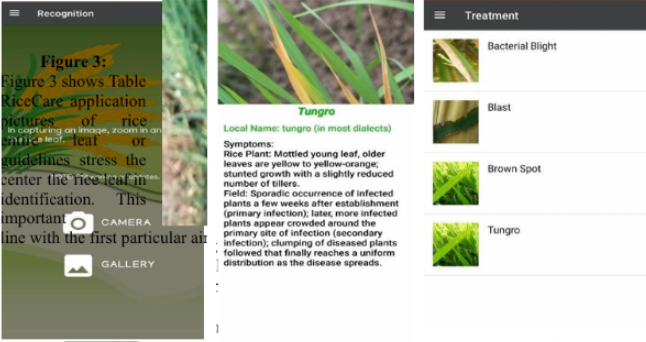
\includegraphics[width=1\textwidth]{chapter2/rice-care-ui.png}
    \caption{RiceCare user interface}
\end{figure}

\subsection{Rice Disease LINE Bot}
\label{subsection:rice-disease-line-bot}

The Rice Disease LINE Bot is an AI-powered chatbot that helps rice farmers detect crop diseases using images taken directly from the field. Integrated into the LINE messaging platform, it allows farmers to send pictures and receive instant disease identification. The system uses deep learning to analyze images and facilitates communication between farmers and experts for better disease management. It also includes a disease knowledge library and a treatment suggestion feature, offering detailed information about the disease and recommendations for effective treatment. The system provides a fast, accessible, and user-friendly solution to support rice farmers in protecting their crops. The user interface is designed to be simple and conversational, where farmers interact with the bot, send images of their crops, and receive instant feedback, along with disease prevention and treatment strategies. (Figure 2.2)

\begin{figure}[h]
    \centering
    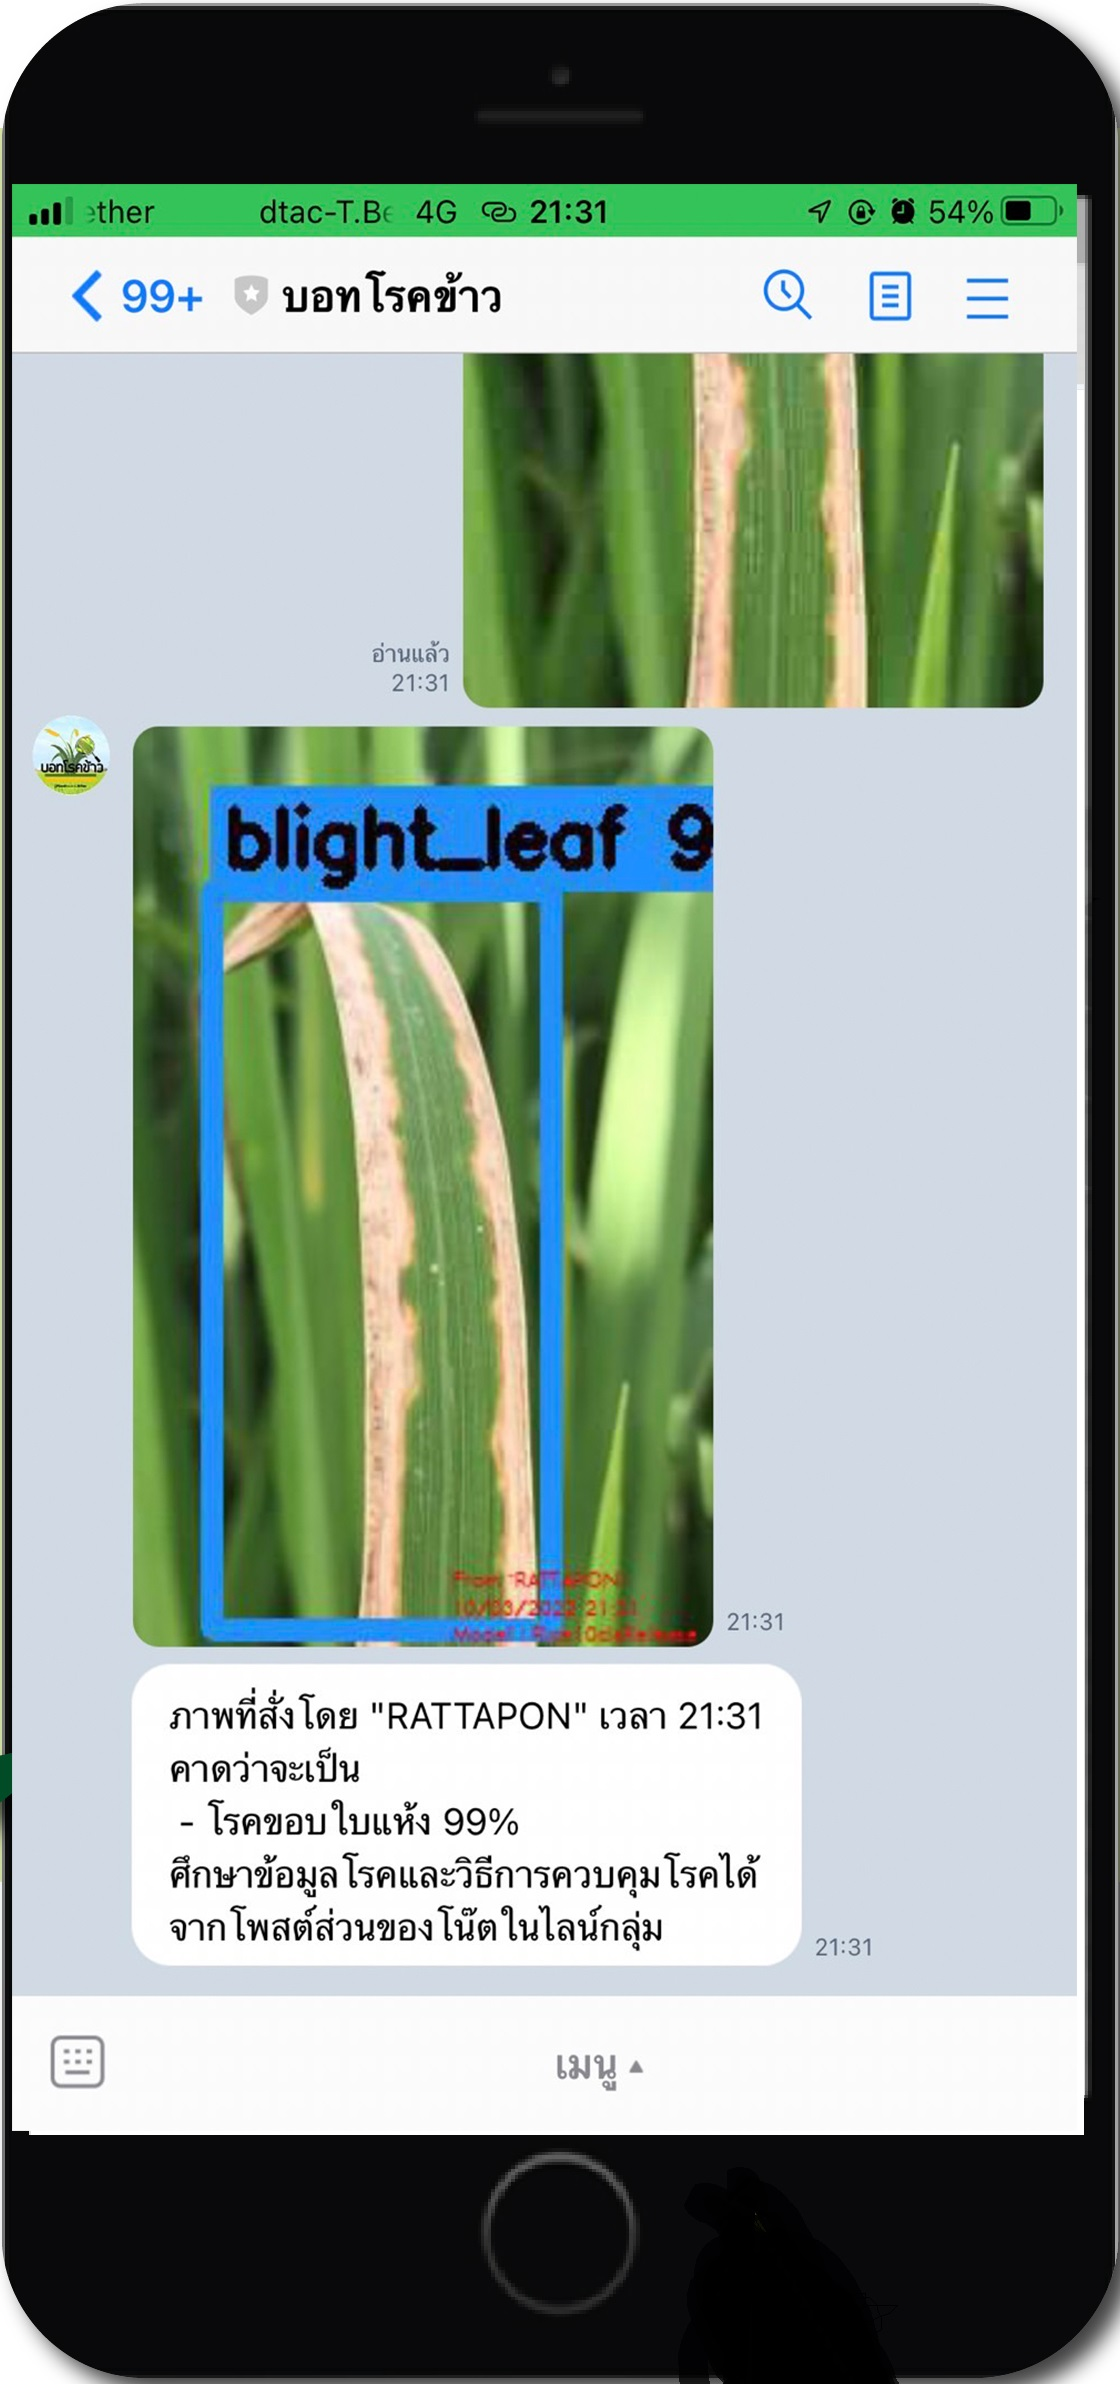
\includegraphics[width=0.4\textwidth]{chapter2/rice-disease-line-bot-ui.jpg}
    \caption{Rice Disease LINE Bot user interface}
\end{figure}

\subsection{Rice Disease Detect}
\label{subsection:rice-disease-detect}

This app allows farmers to take photos of rice plants and diagnose diseases through AI-based image recognition. It provides a user-friendly interface with suggestions for disease management and prevention, but it lacks the real-time communication feature seen in other systems.The user interface is straightforward, where users capture and upload images, and the app processes these images to identify potential diseases. It offers the results along with treatment suggestions for the identified diseases. (Figure 2.3)

\begin{figure}[h]
    \centering
    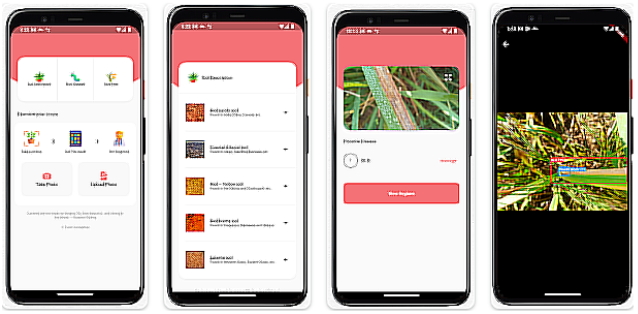
\includegraphics[width=1\textwidth]{chapter2/rice-disease-detect-ui.png}
    \caption{Rice Disease Detect user interface}
\end{figure}

Table 2.1 compares the features of four rice disease detection systems, showcasing their capabilities in disease detection, treatment recommendations, disease libraries, outbreak alerts, and community hubs.

\begin{table}[h!]
    \centering
    \small
    \resizebox{\textwidth}{!}{%
        \begin{tabularx}{\textwidth}{|X|X|X|X|X|}
            \hline
            \textbf{Feature} & \textbf{RiceSafe} & \textbf{RiceCare} & \textbf{Rice Disease LINE Bot} & \textbf{Rice Disease Detect} \\
            \hline
            \textbf{Rice Disease Detection} & Yes (Multimodal AI Model) & Yes (CNNs) & Yes (Deep learning algorithms) & Yes \\
            \hline
            \textbf{Treatment Recommendations} & Yes & Yes & Yes & No \\
            \hline
            \textbf{Disease Library} & Yes & No & Yes & No \\
            \hline
            \textbf{Outbreak Alerts} & Yes (Warns nearby farmers) & No & No & No \\
            \hline
            \textbf{Community Hub} & Yes (Farmers share insights) & No & No & No \\
            \hline
        \end{tabularx}
    }
    \caption{Competitor Comparison Table of Features}
\end{table}

\section{Literature Review}
\label{section:literature-review}

Add a literature review section if it fits with your project.